\documentclass[class=book, crop=false]{standalone}
\usepackage[subpreambles=true]{standalone}
\usepackage{import}
\usepackage[ruled,vlined]{algorithm2e}

\usepackage{amsmath}
\usepackage{amssymb}
\usepackage[margin=1.2in]{geometry}
\usepackage[sorting = none,
            doi = true  %lesedato for url-adresse
            ]{biblatex} %none gir bibliografi i sitert rekkefølge
\addbibresource{reference.bib}
\usepackage{csquotes}
\usepackage{pgfplots}
\pgfplotsset{compat=1.15}

\begin{document}
There are many ways of setting up the state space and reward function that can result in very different behaviour of the agent. This chapter will present results from certain formulation of the reinforcement algorithm. In all cases, deep deterministic policy gradient (DDPG) is used to train the agent. 

\section{Baseline}
It is important to have a baseline to which a trained reinforcement agent can be compared. It is necessary to discuss the physical challenges, and the kind of behaviour that would improve the condition of the electrical grid. As mentioned in \ref{section:problem_description}, the main challenges for the network is that large amount of power must imported and exported out to the external grid in a normal day. Figure \ref{fig:results:demand_and_solar} plots the daily mean solar irradiance signal and power demand used for training the reinforcement agent. The first period that is critical for the grid is when the solar irradiance is at its maximum. The excess solar power produced must be transported out to the grid through many lines due to a large amount of local power production. This can cause overloads in the lines carrying the current and high voltage magnitudes at the bus bars. The second critical period is during peak demand because large amount of energy must be imported from the grid. The problem with importing large amounts of power is potential overloads in the lines, in addition to low voltage magnitudes. A solution to this problem is that profile for the solar production and power demand overlap more. It is not possible to control when the sun shines, but it is possible to manipulate when power is consumed.
\begin{figure}[ht]
    \center
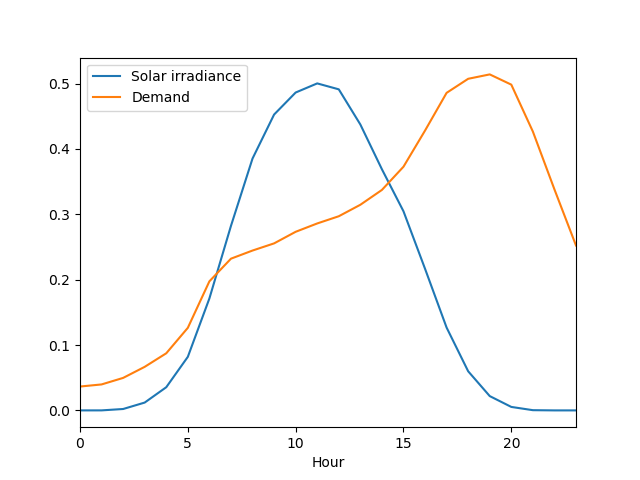
\includegraphics[height=8cm, width=12cm]{figures/demand_and_solar.png}
    \caption[size = 9]{Mean hourly power demand curve and solar irradiance}
    \label{fig:results:demand_and_solar}
\end{figure}

The reinforcement agent is trained with a certain flexibility. It is necessary to inspect what effect the activation of flexibility has on voltage magnitude and line current before a trained agent can be evaluated. Figure \ref{fig:results:increase_demand_current} illustrates the effect activation of flexibility (increasing consumption) has on the current in a critical line. The consumption of active power is increased by 25 \% for all the loads in every hour. The first and second peak in line current correspond, respectively, to the solar peak and the power demand peak. It is clear from the first peak that increasing the consumption decreases the line current. This is because the loads in this period generate so much solar power that they act as producers and not consumers. Increasing the consumption means that less power needs to be transported out to the external grid, which decreases the line current. As a result, the desired behaviour in periods with high solar irradiation is to increase the consumption.

The effect of increasing consumption in the second peak is the opposite of that in the first peak. This is because the loads now act as consumers, and active power must therefore be imported from the external grid. Increasing the consumption in this period simply corresponds to drawing even more power from the external grid, which in turn increases the line current. 

\begin{figure}[ht]
    \center
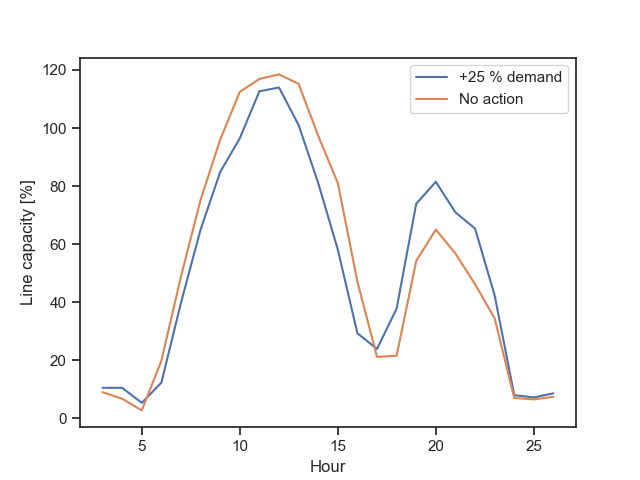
\includegraphics[height=8cm, width=12cm]{figures/increase_demand_current.png}
    \caption[size = 9]{Current in a critical line when increasing load with 25 \% in all hours and regular situation. The line connecting bus 1 and 2 is showed}
    \label{fig:results:increase_demand_current}
\end{figure}


\section{Formulation 1 - Free activation}
A reinforcement agent is trained with reward function that does not include cost of activation. This is not a realistic case, since households that offer flexibility should be compensated for altering their energy profile. This formulation serves to show how an agent would activate flexibility if there was no direct cost associated with altering the power consumption. However, the agent is penalised for changing the total daily energy demand in the power net. Note that it is not penalised for changing the daily consumption at individual loads as long as the total consumption in the network is preserved. The specific reward terms with weights are shown in table \ref{table:results:reward_formulation1}

\begin{table}[ht]
\centering
\caption{Reward terms and weights for formulation 1}
\label{table:results:reward_formulation1}
\begin{tabular}{l|ll}

Cost  & Weight & Comment
\\ 
\hline
Voltage &
1 &
Per-unit values
\\
Current &
$10^{-2}$ &
Percentage of max current 
\\
Activation &
0&
No activation cost
\\
Imbalance &
$10^{-4}$&
Units of energy imbalance is kWh
\\
\hline
\end{tabular}
\end{table}
The state space is constructed to be as small as possible. The state is represented by a 4 hour forecast for both solar irradiance and active power demand. The power demand is assumed equal at each flexible load, so there is not a individual power demand for each load. The total power imbalance for the whole power network is also included. Table \ref{table:results:state_formulation1} summarises the state space

\begin{table}[ht]
\centering
\caption{State used in formulation 1}
\label{table:results:state_formulation1}
\begin{tabular}{l|lll}

State space  & Size & Comment
\\ 
\hline
Solar forecast      &  4  &  4 hour solar forecast
\\ 

Demand forecast    &4 & One 4 hour forecast for all loads
\\ 
Imbalance state & 1  & Total energy imbalance for all loads
\\
\hline
\end{tabular}
\end{table}
The DDPG agent was trained for 100 000 time steps. A complete summary with all hyper-parameters used can be found in appendix ??. Figure \ref{fig:results:configuration1} visualises the actions of the trained agent throughout a day (24 hours) together with the solar irradiance. Because the solar power production in the system is very large, the safety margins for current and voltage are frequently violated. The desired behaviour of the agent is therefore to increase consumption in periods with high solar irradiance. This helps the system because the power is not transported out to the grid, but instead is consumed locally, close to production. Simply put, it is desired that the actions follow the curve of the solar irradiance. 

\begin{figure}[ht]
    \center
    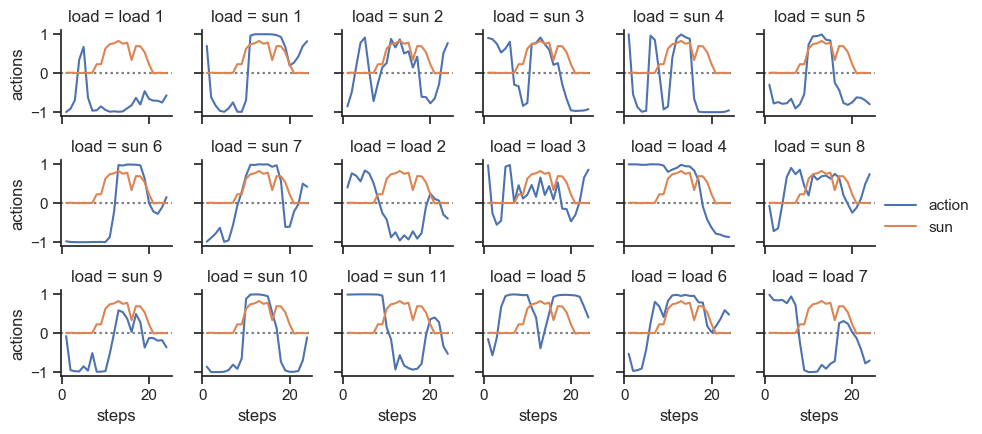
\includegraphics[height=8cm, width=15cm]{figures/configuration1.png}
    \caption[size = 9]{Activation of flexibility at the different flexible loads of the trained DDPG throughout a day. The orange line is the solar irradiance during the day, which is the same for all loads. The actions in blue is the activation of flexibility. Action = 1 means that the flexible load increases its power consumption with 10 \%, while action = -1 means that it decreases its power consumption with 10 \%}
    \label{fig:results:configuration1}
\end{figure}
By inspecting figure \ref{fig:results:configuration1} it is clear that the agent activates flexibility in times with much solar production for several of the loads. The plot \texttt{load = sun 10} in the bottom row is plotted alone in figure \ref{fig:results:configuration1_follows_sun}, and clearly follows this pattern. The agent increases its power consumption during periods with high solar production, and reduces it later to ensure that the energy consumption is shifted, and not altered in absolute magnitude.

\begin{figure}[ht]
    \center
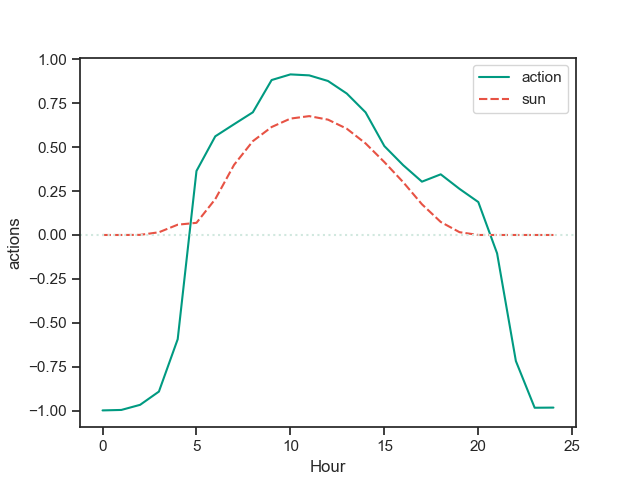
\includegraphics[height=8cm, width=12cm]{figures/configuration1_follows_sun.png}
    \caption[size = 9]{Action of the agent and solar profile during a day. The consumed power is increased in periods with high solar production}
    \label{fig:results:configuration1_follows_sun}
\end{figure}

\begin{figure}[ht]
    \center
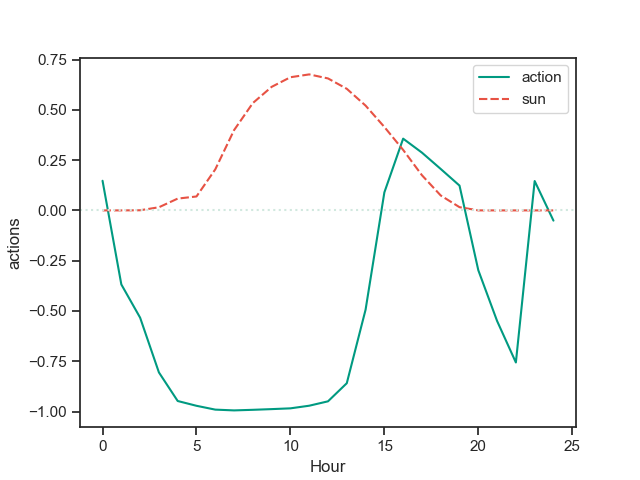
\includegraphics[height=8cm, width=12cm]{figures/configuration1_negative_actions.png}
    \caption[size = 9]{Action of the agent and solar profile during a day}
    \label{fig:results:configuration1_negative_actions}
\end{figure}

 The first plot in the top row \texttt{load = load 1} is plotted larger in figure \ref{fig:results:configuration1_negative_actions}, and show some peculiar behaviour. Clearly, the actions do not follow the solar profile that day, but are negative most of the day. This behaviour could be a result of how the reward function is defined in this configuration. The agent is penalised according to the total energy imbalance in the system, not at individual loads. As a result, if the energy imbalance is +1 MWh at one load and -1 MWh at another load, they perfectly cancel each other, and the agent is not penalised. From the agent's perspective, the system is in energy balance, although individual loads may have a large absolute energy imbalance. This illustrates the problem with constructing state variable that accounts for the system as a whole, and not individual loads. The agent uses the same strategy consistently at this load. It appears as if this load functions as a energy balance, whose main job is to ensure that the total power imbalance in the grid is kept as small as possible. However, the behaviour of the agent gives a negative energy imbalance, as seen in figure \ref{fig:results:configuration1_energy_imbalance}. The agent controls a 200 hour long episode, and it is evident that the energy imbalance quickly decreases and reaches an equilibrium around -13 MWh. The agent prefers to decrease the total consumption in the system, which is an unexpected behaviour. In fact, the expected behaviour is that the agent would increase the energy imbalance of the system because it consumes more power in periods with high solar power. It may indicate that the reward function is not appropriately constructed. More specifically, the energy imbalance cost is designed to reward the agent every time the energy imbalance decreases in absolute magnitude. A problem with this approach could be that the agent is not penalised for having a large absolute power imbalance. The reward function considers an energy imbalance transition from -11 MWh to -10 MWh equally good as a transition from -1 MWh to 0 MWh.
 
\begin{figure}[ht]
    \center
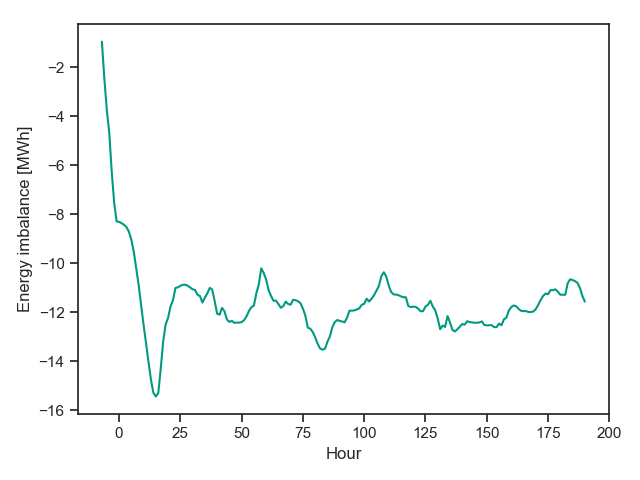
\includegraphics[height=8cm, width=12cm]{figures/configuration1_imbalance.png}
    \caption[size = 9]{Total energy imbalance at all the flexible loads when the agent control a 200 hour episode}
    \label{fig:results:configuration1_energy_imbalance}
\end{figure}
Figure ?? plots the rewards given in every step in a 200-hour long episode for the trained agent and an agent taking no actions. The curve corresponding to no agent is equivalent to a scenario with no reinforcement algorithm, since no actions are taken. By definition, the imbalance cost will be 0 for the no-action scenario because it never alters the energy consumption. Consequently, the no action scenario is only penalised based on violation of safety margins on voltage and line current. The rewards illustrate some clear weaknesses in the trained agent. The original goal of the agent is to take actions to prevent violations of voltage and line current safety margins. Those periods correspond to the spikes in figure ??, which is when the solar power production is high. It is evident that the trained agent actually is worse in those critical periods, and has not learned the desired behaviour. The trained agent occasionally gets a positive rewards when the energy imbalance in the system decreases. On average, the total episodic reward is about the same, but it is clear that the reward function is not well tuned. The agent should be more penalised for violating safety margins for voltage and line current.



\end{document}